% Created 2019-11-26 Tue 04:01
% Intended LaTeX compiler: pdflatex
\documentclass[fleqn]{article}
\usepackage[utf8]{inputenc}
\usepackage[T1]{fontenc}
\usepackage{graphicx}
\usepackage{grffile}
\usepackage{longtable}
\usepackage{wrapfig}
\usepackage{rotating}
\usepackage[normalem]{ulem}
\usepackage{amsmath}
\usepackage{textcomp}
\usepackage{amssymb}
\usepackage{capt-of}
\usepackage{hyperref}
\usepackage{minted}
\usepackage{../homework}
\DeclareSIUnit \VA { VA }
\DeclareSIUnit \VAR { VAR }
\author{Lewis Collum}
\date{Updated: \today}
\title{EE331 Fall 2019 HW \jobname}
\hypersetup{
 pdfauthor={Lewis Collum},
 pdftitle={EE331 Fall 2019 HW \jobname},
 pdfkeywords={},
 pdfsubject={},
 pdfcreator={Emacs 26.3 (Org mode 9.1.9)}, 
 pdflang={English}}
\begin{document}

\maketitle

\section*{(1)}
\label{sec:org2d956c3}
First we encapsulate values that are given in python
dictionaries. 
\begin{minted}[bgcolor=codeBackground]{python}
import numpy
import matplotlib.pyplot as pyplot
import pint
unit = pint.UnitRegistry()

terminal = {
    'power': 120 * unit.kW,
    'voltageRated': 266 * unit.V
}

stator = {
    'currentRated': 180 * unit.A,
    'impedance': (0.05 + 1.5j) * unit.ohms
}

field = {}
\end{minted}

We are assuming the motor is running at its rated voltage. With this
assumption, we get the current through the stator.
\begin{minted}[bgcolor=codeBackground]{python}
stator['current'] = (terminal['power']/3/terminal['voltageRated']).to('A')
print(f"\(I_s = {stator['current']:.2fLx}\)")
\end{minted}

\(I_s = \SI[]{150.38}{\ampere}\)

Since we know the rated current, we can find out the max imaginary
stator current.
\begin{minted}[bgcolor=codeBackground]{python}
stator['currentMaxImaginary'] = numpy.sqrt(stator['currentRated']**2 - stator['current']**2)
print(f"\(\max{{(I_m(I_s))}} = {stator['currentMaxImaginary']:.2fLx}\)")
\end{minted}

\(\max{(I_m(I_s))} = \SI[]{98.93}{\ampere}\)

We will use the max imaginary current to establish a range for our
v-curve.
\begin{minted}[bgcolor=codeBackground]{python}
imaginaryRange = 1j*stator['currentMaxImaginary'] * numpy.linspace(-1, 1, 21, endpoint=True)
stator['currents'] = stator['current'] + imaginaryRange
\end{minted}

Now we can calculate the field current, \(I_f\), for each stator
current in our \texttt{stator['currents']} array.

\begin{minted}[bgcolor=codeBackground]{python}
field['voltages'] = (stator['currents']*stator['impedance'] + terminal['voltageRated']).to('V')
field['currents'] = (abs(field['voltages']) / (30*unit.ohms)).to('A') #Given in problem statement
\end{minted}

Finally, we plot stator currents vs field currents.
\begin{center}
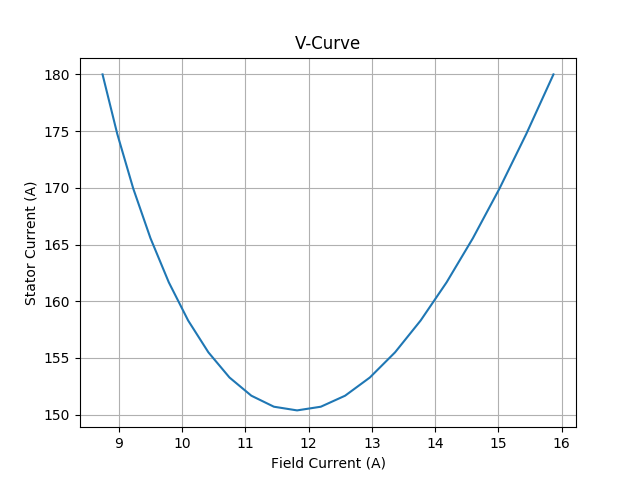
\includegraphics[width=0.6\linewidth]{vcurve.png}
\end{center}

\section*{(2)}
\label{sec:orgca01e5a}
\subsection*{(a) Find \(P_{max}\) at \(E_f = 19.5\si{kV}\)}
\label{sec:orgc621776}

Assuming \(R_s, R_{sys} \ll X_{sys} \ll X_s\):
\[X_T = X_s + X_{sys} = \SI[]{0.80}{\ohm}\]

And, given:
\[V_{bus} = \SI[]{13.00}{\kilo\volt}\]
\[E_f = \SI[]{19.50}{\kilo\volt}\]

The maximum output power of the generator is obtained when \(\delta = 90^{\circ}\).
\[P_{e,max} = \frac{3 E_f V_{bus}}{X_T}\sin{90^{\circ}} = \boxed{ \SI[]{950.63}{\mega\watt} }\]

\subsection*{(b)}
\label{sec:org5f0cd4e}
\[\delta = \sin^{-1}{\frac{700\si{MW}}{P_{e,max}} = \boxed{ \SI[]{47.42}{\degree} }\]

\subsection*{(c)}
\label{sec:orge5a70f5}
We apply the current \(\delta\) to the field voltage at \(\delta =
   90^{\circ}\) to get \(E_f\).
\[E_f = 19.50 \angle 47.42^{\circ} \si[]{\kilo\volt}\]

Now, to get the stator current, \(I_s\),
\[E_f = I_s \cdot X_T + V_{bus}\]

\[\to I_s = \frac{E_f - V_{bus}}{X_T} = 17.95 \angle -0.77^{\circ} \si[]{\kilo\ampere}\]

Finally, we get the terminal voltage, \(V_t\).
\[V_t = I_s \cdot X_{sys} + V_{bus}\]

\[V_t = \boxed{ 14.79 \angle -0.09^{\circ} \si[]{\kilo\volt} }\]

\subsection*{(d)}
\label{sec:org1eb70c5}


\[S_t = \SI[]{796.66+9.44j}{\mega\VA}\]
\[Q_t = \boxed{ \SI[]{9.44}{\mega\VAR} }\]

\subsection*{(e)}
\label{sec:org17ebba3}
\[\delta = \sin^{-1}{\frac{200\si{MW}}{P_{e,max}} = \boxed{ \SI[]{12.15}{\degree} }\]

\section*{(3)}
\label{sec:org5a3d9a0}
\subsection*{(a) Calculate Motor Slip}
\label{sec:org406a9e0}
\[s = \frac{\omega_2}{\omega_1} = \frac{\omega_1 - p_p \omega_r}{\omega_1}\]
\[\omega_1 = \SI[]{376.99}{\radian\per\second}\]
\[\omega_r = \SI[]{91.63}{\radian\per\second}\]
\[s = \frac{\omega_1 - p_p\omega_r}{\omega_1} = \boxed{ \SI[]{0.03}{} }\]

\subsection*{(b) \(I_1\), \(I_2\)}
\label{sec:org611567b}
\[Z_{eq} = R_1 + jX_1 + (\frac{R_2'}{s} + jX_2')||jX_m = \SI[]{1.88+0.75j}{\ohm}\]
\[I_1 = \frac{V_1}{Z_{eq}} = \boxed{ 131.13 \angle -21.76^{\circ} \si[]{\ampere} }\]
\[E_1 = 251.15 \angle -5.01^{\circ} \si[]{\volt}\]
\[I_2' = \frac{E_1}{R_2'/s + jX_2'} = \boxed{ 126.20 \angle -10.78^{\circ} \si[]{\ampere} }\]

\subsection*{(c) Motor Efficiency}
\label{sec:org5a760ba}
\[P_1 = \Re{(3V_1I_1^{*})} = \SI[]{97.18}{\kilo\watt}\]
\[P_{es} = \Re{(3E_1I_2'^{*})} = \SI[]{94.60}{\kilo\watt}\]
\[P_m = (1-s)P_{es} = \SI[]{91.97}{\kilo\watt}\]
\[\eta = \frac{P_m}{P_1} = \boxed{ \SI[]{0.95}{} }\]

\subsection*{(d)}
\label{sec:org400ca36}
Assuming no mechanical loss, \(P_e = P_m\)
\[T_e = \frac{P_e}{\omega_r} = \boxed{ \SI[]{1.00}{\kilo\watt\second\per\radian} }\]
\section*{(4)}
\label{sec:orge746861}
\[Z_{eq} = R_1 + jX_1 + (\frac{R_2'}{s} + jX_2')||jX_m + Z_{th} = \SI[]{0.14+0.51j}{\ohm}\]
\[I_1 = \frac{V_{src}}{Z_{eq}} = \boxed{ 526.48 \angle -74.24^{\circ} \si[]{\ampere} }\]
\[V_t = V_{src} - I_1Z_{th} = \boxed{ 215.59 \angle 1.21^{\circ} \si[]{\volt} }\]

\section*{(5)}
\label{sec:org7567bc8}
\subsection*{(a) Slip}
\label{sec:orgb91e273}
\[\omega_1 = \SI[]{376.99}{\radian\per\second}\]
\[\omega_r = \SI[]{193.73}{\radian\per\second}\]
\[\omega_2 = \SI[]{-397.94}{\radian\per\second}\]
\[s = \boxed{ \SI[]{-1.06}{} }\]
\end{document}